\documentclass[zad,zawodnik,en]{sinol}
  \signature{boi012}
  \id{gat}
  \title{Gates}
  \author{Linas Petrauskas}
  \etap{}
  \day{1}
  \date{19--04--2008}
  \RAM{96}                %% Memory limit -- can be skipped in a proposal
  \Time{4}              %% Time limit --  can be skipped in a proposal
  \def\sinolContestLogo{boi08-logo}
  \iomode{stdin}
  \pagestyle{fancy}
  \history{08.03.2008}{[JR] Redakcja}{1.0}
  \history{27.03.2008}{[WT] Uzupelnienie limitow}{1.1}
  \history{06.04.2008}{[MP] Change of guaranteed set of points, minor changes}{1.2}

\begin{document}
  \begin{text}%
    After many years of working as a software developer you have decided to try
    something entirely different, and started looking at random job offers.
    The one that really caught your eye was a job in fish farming (a form of
    aquaculture).
    'Cool!', you thought, and besides, fish are
    nice creatures.
    So you applied, got accepted, and today is your first day at work.

    Your boss has already assigned you a task.
    You have to isolate one water reservoir from another.
    After looking at some schemes you've been given, here's what you've figured
    out.

    The two water reservoirs are connected by several channels.
    Each channel has two gates.
    The channel is open when both gates are open, and is closed otherwise.
    The gates are controlled using switches.
    The same switch may operate several gates, but each gate is operated by
    exactly one switch.
    It is possible that both gates on a channel are controlled by the same switch
    and that a switch controls no gates.
    \begin{center}
      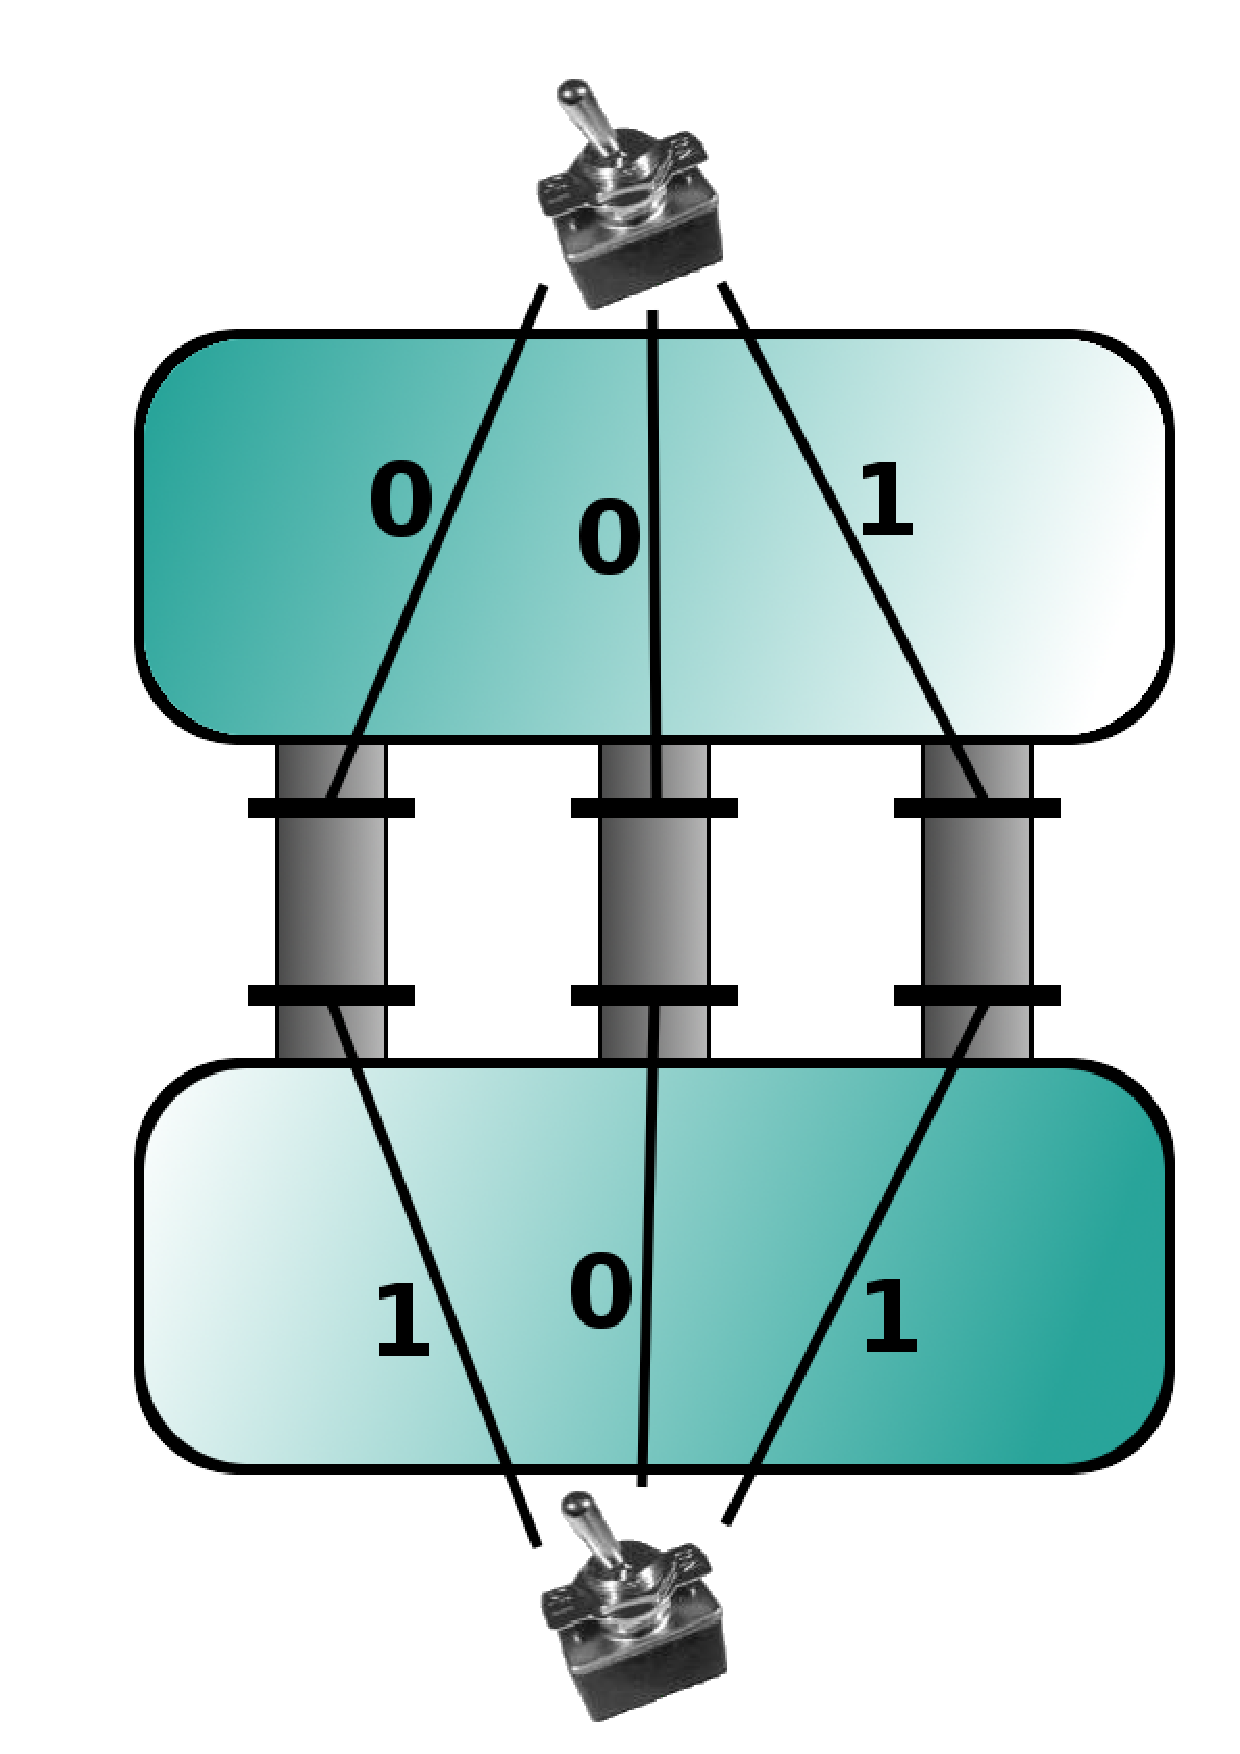
\includegraphics[width=5cm]{gates}\\
      \textit{Example with three channels and two switches.}
    \end{center}
    The switch may operate the gate in one of two ways:
    \begin{itemize}
      \item
        the gate is open when the switch is on, and is closed when the switch is off,
      \item 
        the gate is closed when the switch is on, and is open when the switch is off.
    \end{itemize}

    After playing a bit with the switches you suddenly realize that your
    programming experience will come in very handy.
    Write a program that, given the configuration of gates and switches,
    determines whether it is possible to close all channels, and if it is,
    then finds a state of every switch in one such valid configuration.

    \section{Input}
      The first line of the standard input contains two integers $n$ $(1 \le n \le 250\,000)$ 
		and $m$ $(1 \le m \le 500\,000)$, the number of channels and switches respectively.
      Switches are numbered from $1$ to $m$. Additionally, in test cases worth at least $30$\% points,
		$n$ will not exceed $40$ and $m$ will not exceed $20$.
		

      The following $n$ lines describe channels, each channel is described by 
      a separate line containing four integers:
      $a$, $s_a$, $b$, $s_b$.
      Numbers $a$ and $b$ represent switches ($1\le a,b\le m$) that operate gates
      of this channel.
      Numbers $s_a$ and $s_b$ can be either $0$ or $1$ and correspond to the described
      operation modes: $s_i=0$ means that the gate is closed if and only if the
      switch $i$ is off and $s_i=1$ means that the gate is closed if and only
      if the switch $i$ is on.

    \section{Output}
      If it is possible to close all the channels, the standard output should contain
      $m$ lines.
      Line $i$ should contain $0$, if switch $i$ should be off, and $1$ if
      switch $i$ should be on.
      If there are many possible solutions, your program may output any of them.

      If it is impossible to close all channels, your program should output one
      line, containing a single word \texttt{IMPOSSIBLE}.

  \makecompactexample

  \twocol{
    and for the input data:
  \iffileexists{\sinolTestIn/\ID0a.in}{%
    \includefile{\sinolTestIn/\ID0a.in}
  }{
    \includefile{\ID0a.in}
  }
  }{
    the correct result is:
    \iffileexists{\sinolTestOut/\ID0a.out}{%
      \includefile{\sinolTestOut/\ID0a.out}
    }{
      \includefile{\ID0a.out}
    }
  }
  \noindent
  The first example corresponds to the picture from the task description.
  \end{text}
\end{document}
